% main.tex — só preâmbulo e \input. Nenhum conteúdo nasce aqui.
% preambulo.tex — cada \usepackage comentado com a regra do guia que atende.
% Fonte de todas as remissões: auditoria/parametros_guia.md (página impressa do guia).
%
% Decisão de classe (Fase 2, registrada em auditoria/log.md): abntex2, não formatação
% manual. Justificativa: abntex2 já nasce configurado para as margens, corpo de fonte
% e entrelinhas que o guia pede (§1 de parametros_guia.md — 3/2cm, 12pt, 1,5 entrelinhas),
% e resolve de fábrica a maior parte dos elementos pré-textuais (capa, folha de rosto,
% ficha catalográfica, resumo, listas, sumário — §7). Onde o guia diverge do
% comportamento padrão do pacote, o pacote é sobrescrito e a divergência vai para o log
% (R-3: guia vence pacote). Montar tudo à mão custaria mais do que essas sobrescritas.

\documentclass[
  12pt,          % corpo do texto — guia p. 12 ("fonte tamanho 12 para o texto")
  a4paper,       % papel A4 (210x297mm) — guia p. 12
  oneside,       % entrega só digital (PDF); guia permite anverso-only para textual/
                 % pós-textual (p. 13) e não exige twoside para TCC de graduação.
                 % Único caso de "verso" no guia é a ficha catalográfica atrás da folha
                 % de rosto (p. 13), tratado como página própria em sequência, não como
                 % impressão física frente/verso — ver DECISÃO em auditoria/log.md.
  chapter=TITLE, % títulos de capítulo em caixa alta + negrito — confirmado no exemplo
                 % real de sumário do próprio guia (Figura 11, p. 20: "2 A BIBLIOTECA"
                 % em maiúsculas e negrito). NÃO usar section=TITLE: no mesmo exemplo,
                 % os títulos de nível 2 ("2.1 História") aparecem em negrito, mas
                 % SEM caixa alta. O negrito em si NÃO é automático (achado C2/Fase 8,
                 % ver bloco de correção logo abaixo do \documentclass) — a suposição
                 % original aqui estava errada.
  english,       % hifenização auxiliar (títulos/termos em inglês no corpo)
  brazil,        % idioma principal do documento
]{abntex2}

% memhfixc: abntex2 é baseado em memoir, que já carrega hyperref internamente;
% memoir+hyperref têm uma interação conhecida de contadores/âncoras que produz
% destinos de página duplicados (ex. "page.1" repetido entre capa e folha de
% rosto) — memhfixc é o patch oficial do próprio memoir para isso, e precisa vir
% DEPOIS de hyperref já estar carregado (por isso aqui, logo após \documentclass,
% já que abntex2.cls carrega hyperref internamente antes deste ponto).
\usepackage{memhfixc}

% Negrito em título de capítulo e de seção primária (guia p. 21-22 e Figura 11,
% p. impressa 20) — achado C2/Fase 8 (ver auditoria/log.md §21): abntex2.cls
% define \ABNTEXchapterfont e \ABNTEXsectionfont como \sffamily puro, sem
% \bfseries em nenhum dos dois, e \setsecheadstyle/\chaptitlefont usam essas
% macros diretamente — nenhum nível de título sai em negrito por padrão. Só a
% capa (\imprimirtitulo) tem \bfseries embutido manualmente na classe, prova de
% que o negrito é intencional em outros títulos de destaque, só ausente aqui.
% \ABNTEXsubsectionfont/\ABNTEXsubsubsectionfont, na classe, são definidas como
% referências a \ABNTEXsectionfont (não cópias) — por isso são redefinidas aqui
% também, de forma independente, sem \bfseries, para NÃO herdar o negrito que
% \ABNTEXsectionfont ganha logo abaixo (guia: só seção 1ª/2ª em negrito).
\renewcommand{\ABNTEXchapterfont}{\sffamily\bfseries}
\renewcommand{\ABNTEXsectionfont}{\sffamily\bfseries}
\renewcommand{\ABNTEXsubsectionfont}{\sffamily}
\renewcommand{\ABNTEXsubsubsectionfont}{\sffamily}

% Mesmo defeito, mesma causa, achado no recheque do fix acima (Fase 8, ver
% auditoria/log.md §21): no Sumário, \cftchapterfont/\cftsectionfont
% (abntex2.cls linhas 520-529) são \bfseries, mas \cftsubsectionfont/
% \cftsubsubsectionfont só ajustam \normalsize/\small, sem nunca desligar o
% negrito com \mdseries — confirmado por `pdffonts`: a página do Sumário só
% usa a fonte Bold, em todo nível, do capítulo à subsubseção. Corrigido do
% mesmo jeito: \mdseries explícito só nesses dois níveis, sem tocar
% \cftchapterfont/\cftsectionfont (que devem continuar em negrito).
\renewcommand{\cftsubsectionfont}{\normalsize\mdseries}
\renewcommand{\cftsubsubsectionfont}{\small\mdseries}

% ---------------------------------------------------------------------------
% Idioma e codificação
% ---------------------------------------------------------------------------
\usepackage[T1]{fontenc}
\usepackage[utf8]{inputenc}
\usepackage{lmodern}         % fallback de fonte vetorial; substituído por mathptmx abaixo
\usepackage{mathptmx}        % Times New Roman (equivalente PostScript) — guia p. 12
                              % permite Arial OU Times New Roman; Times é o padrão de
                              % fábrica do ecossistema abntex2/ABNT em pdfLaTeX.

% ---------------------------------------------------------------------------
% Citação (NBR 10520:2023) e referências (NBR 6023:2025)
% ---------------------------------------------------------------------------
\usepackage[
  alf,
  abnt-etal-text=it,         % *et al.* em itálico — regra já vigente no texto-fonte
  abnt-doi=doi,              % NÃO expande "Disponível em:" para um link
                              % https://dx.doi.org/... — testado com
                              % abnt-doi=expand e não teve efeito nenhum: o
                              % ramo de compose.url() que consultaria essa
                              % opção só roda com abnt.url.package=0, e este
                              % documento usa abnt.url.package=1 (pacote url
                              % ativo, citeoption "abnt-url-package=url" já
                              % disparada pelo próprio abntex2cite), cujo
                              % ramo ignora abnt-doi por completo — achado
                              % empírico, não vale a pena outro patch de .bst
                              % só por isso. A cláusula "DOI: 10.xxxx."
                              % separada que o guia pede (p. 34: "...ano. DOI
                              % (se houver). Disponível em:...") NÃO existe
                              % nesta versão do abntex2-alf.bst nem como
                              % opção — patch local em
                              % latex/bst/abntex2-alf-tg1.bst, função
                              % format.url (achado do autor, ver
                              % auditoria/log.md §25). "Disponível em:"
                              % continua mostrando "doi:10.xxxx" cru, o que
                              % não é vedado pelo guia (nota técnica de
                              % parametros_guia.md §9.1: os sinais < > são
                              % convenção tipográfica, não texto do URL).
  abnt-full-initials=yes,   % prenomes por extenso na lista — regra do projeto
                              % ("Prenomes por extenso em todas as entradas").
                              % Default do pacote é abreviar (achado empírico:
                              % 1ª compilação saiu "ACHTERBERG, T." em vez de
                              % "ACHTERBERG, Tobias" — ver auditoria/log.md).
  tg1-cite-style,            % "(Author, YEAR)" — inicial maiúscula na chamada,
                              % caixa alta só na lista (NBR 10520:2023, já em
                              % vigor nos dois capítulos-fonte). Chave própria,
                              % definida em referencias.bib, citando um valor
                              % que o pacote embutido também define, mas sob uma
                              % chave que colide (achado empírico, auditoria/
                              % log.md Fase 4: BibTeX trata chaves de citação
                              % como insensíveis a maiúscula/minúscula, e
                              % "abnt-cite-style=AUTHORYEAR" colide com
                              % "...=AuthorYEAR", sempre resolvendo para a
                              % primeira, caixa alta — daí a chave própria).
                              % Passada como OPÇÃO DE PACOTE, não via
                              % \citeoption direto: \citeoption chamado no
                              % preâmbulo escreve no .aux antes de \@auxout
                              % existir e é descartado em silêncio; como opção
                              % de pacote, o próprio abntex2cite adia a chamada
                              % para \AtBeginDocument, quando o .aux já existe.
]{abntex2cite}
% Estilo alfabético (autor-data) — catálogo já usa esse sistema em todo o texto-fonte
% (ex. "(FORREST et al., 2019)" na lista, "(Forrest et al., 2019)" em texto), não o
% sistema numérico.

% ---------------------------------------------------------------------------
% Figuras, quadros e tabelas — legenda acima, fonte abaixo (guia p. 23-24)
% ---------------------------------------------------------------------------
\usepackage{graphicx}
\usepackage{float}
\usepackage{caption}
\usepackage{placeins}       % \FloatBarrier — achado do autor, 13/08/2026 (ver
                              % auditoria/log.md §25): um Quadro[htbp] adiado
                              % (Quadro 7) drenava a página seguinte inteira e
                              % empurrava a Figura 3 (mesmo com [H]) 2 páginas
                              % para frente. \FloatBarrier força os flutuantes
                              % pendentes de uma seção a resolver antes da
                              % próxima, sem alterar nenhuma legenda/numeração.

% Legenda ACIMA do conteúdo para figuras — diverge do padrão de fábrica do LaTeX
% (que põe legenda de figura abaixo). DIVERGÊNCIA guia×pacote, registrada em
% auditoria/log.md: o guia (p. 23) manda identificação "na parte superior" para
% qualquer tipo de ilustração, sem exceção para figuras.
\floatstyle{plaintop}
\restylefloat{figure}
\restylefloat{table}

% Ambiente \quadro distinto de \table — plano exige que a diferença entre Quadro
% (qualitativo) e Tabela (numérico) seja estrutural, não editorial (prompt, §5).
% Numeração corrida (sem "within"), não por capítulo: o texto-fonte já audita
% Quadro 1..11 (mais 3a e 7a) como sequência única do documento, não "Quadro
% 3.1" — ver auditoria/log.md, Fase 3.
\newfloat{quadro}{htbp}{loq}
\floatname{quadro}{Quadro}
\floatstyle{plaintop}
\restylefloat{quadro}

% Figura e Tabela também numeradas de forma corrida, pelo mesmo motivo: o
% texto-fonte usa "Figura 1/2/3" e "Tabela 1" flat, não escopado por capítulo
% (que é o padrão de fábrica do memoir/abntex2 para relatórios multi-capítulo).
\counterwithout{figure}{chapter}
\counterwithout{table}{chapter}
% Equações também: numeração corrida, não "(3.1)" por capítulo. Só as 2
% equações efetivamente referenciadas em texto (PL, MILP) são numeradas — as
% outras 5 do Cap. 3 usam align*/equation* (guia p. 22: numera-se "só quando
% necessário"; achado C2/Fase 8, ver auditoria/log.md §19).
\counterwithout{equation}{chapter}

% "Título de seção primária inicia em página ímpar" (guia p. 12) é regra de
% NUMERAÇÃO, independente de oneside/twoside (que é só sobre impressão física).
% A opção nativa \openright da memoir NÃO resolve isso aqui: seu
% \clearforchapter (memoir.cls) só insere a página em branco sob \if@twoside —
% em oneside ele degrada para um \clearpage comum, achado empírico (Fase 8).
% Reimplementado manualmente, sem depender de \if@twoside: mantém oneside
% (decisão da Fase 2, entrega só digital) e ainda força \chapter a cair em
% página ímpar. Achado C2/Fase 8, ver auditoria/log.md §19.
\makeatletter
\renewcommand{\clearforchapter}{%
  \clearpage
  \ifodd\value{page}\else
    \hbox{}\thispagestyle{empty}\newpage
  \fi
}
\makeatother

% Comando \fontenota — a "Fonte:" abaixo do conteúdo é elemento obrigatório mesmo em
% produção do próprio autor (guia p. 23: "elaborado pelo próprio autor"). Não é o
% \caption padrão do LaTeX (que abntex2 já usa para a legenda de cima); é uma segunda
% linha, centralizada, fonte reduzida, adicionada manualmente dentro de cada float.
\newcommand{\fontenota}[1]{%
  \par\nobreak
  {\small\centering Fonte: #1\par}%
}
% \par antes do grupo: sem isso, uma tabela/quadro estreito (que não ocupa a
% largura inteira, ex. a Tabela 1 de McNemar) não força quebra de linha
% sozinho, e a linha "Fonte:" aparece colada ao lado do conteúdo em vez de
% abaixo — achado empírico, corrigido aqui de uma vez para todos os usos.

\captionsetup{
  labelsep=endash,   % "travessão" entre número e título — guia p. 23 ("travessão")
  font=small,        % fonte reduzida para legendas — guia p. 12 (10/11 para legendas)
  justification=centering,
}

% ---------------------------------------------------------------------------
% Equações numeradas à direita, só as referenciadas — guia p. 22
% ---------------------------------------------------------------------------
\usepackage{amsmath}
\usepackage{amssymb}
% amsmath numera à direita por padrão; equações sem \label/\eqref não citadas
% permanecem sem número visível de fato relevante — a disciplina de "só numerar o
% que é referenciado" é aplicada na redação (Fase 3), não no preâmbulo.

% ---------------------------------------------------------------------------
% Apoio geral
% ---------------------------------------------------------------------------
\usepackage{indentfirst}
% Recuo de primeira linha de parágrafo — o guia NÃO especifica um valor de recuo em
% nenhuma das 66 páginas lidas (só especifica o recuo de 4cm para citação longa,
% guia p. 25). DECISÃO (não DIVERGÊNCIA, porque o guia é silente, não contraditório):
% usar o recuo padrão do abntex2 (1,25cm), prática corrente ABNT. Ver auditoria/log.md.

\usepackage{microtype}       % justificação tipográfica fina — não normativo, só qualidade
\usepackage{xcolor}          % suporte de cor para BPMN e destaques pontuais
\usepackage{booktabs}        % regras horizontais para a Tabela de McNemar (única Tabela)
\usepackage{tabularx}        % colunas de largura flexível — os 13 Quadros do Cap. 3
                              % têm células de texto longo, não cabem em tabular fixo
\usepackage{array}           % suporte a especificadores de coluna customizados (p{})

% hyperref já é carregado internamente pelo abntex2 (via bookmark.sty) — carregá-lo
% de novo com opções próprias causa "Option clash". Ajuste feito por \hypersetup,
% não por novo \usepackage. Não é exigido pelo guia; só navegação interna do PDF
% (sumário clicável, remissões), sem alterar a aparência impressa do documento.
% plainpages=false: sem isso, hyperref nomeia âncoras de página pelo valor impresso
% de \thepage, que o abntex2 mantém intencionalmente parado durante \pretextual
% (guia p. 12: "folhas pré-textuais devem ser contadas... mas não numeradas") —
% duas páginas físicas distintas (capa, folha de rosto) ficam com o mesmo \thepage
% e colidem no nome da âncora ("destination... page.1... duplicate ignored").
% plainpages=false usa o número físico absoluto para o nome da âncora em vez do
% valor impresso, resolvendo a colisão sem alterar a numeração visível do documento.
% Fonte do diagnóstico: TeX FAQ, "pdfTeX destination ... ignored"
% (https://texfaq.org/FAQ-hyperdupdest).
\hypersetup{colorlinks=false, hidelinks, plainpages=false, pageanchor=false}

% ---------------------------------------------------------------------------
% Metadados do documento — preenchidos em pretextual/dados.tex (Fase 7)
% ---------------------------------------------------------------------------
% \autor, \titulo, \instituicao etc. ficam num arquivo à parte porque dependem de
% dados que ainda não foram confirmados (nome completo do autor, título exato,
% orientador) — ver PENDÊNCIA em auditoria/log.md. Não fabricar aqui (R-2).

% pretextual/dados.tex — metadados do documento (comandos abntex2).
%
% R-2 (zero dado de memória): autor, orientadora e curso confirmados
% diretamente pelo autor em 09/08/2026 (auditoria/log.md, Fase 8); título
% confirmado diretamente pelo autor em 14/08/2026 (auditoria/log.md §26) —
% nenhum dos dois é inferência. RESUMO (NBR 6028:2021) ainda não está pronto
% para esta rodada de TG1 — fica fora do escopo desta fase por decisão do
% autor, não fabricado.

\titulo{Plataforma multiagente \textit{low-code} para formulação e resolução de problemas de programação linear e linear inteira mista a partir de descrições em língua portuguesa}
\autor{Thiago Bibiano da Silva}
\instituicao{Universidade Federal do ABC}
\local{Santo André}
\data{\the\year}
\orientador{Carolina Corrêa de Carvalho}

\tipotrabalho{Trabalho de Graduação}
\preambulo{%
  Trabalho de Graduação apresentado ao curso de Bacharelado em Engenharia de
  Gestão da Universidade Federal do ABC como requisito parcial para obtenção
  do título de Bacharel em Engenharia de Gestão.%
}


\begin{document}

\pretextual
  % pretextual/capa.tex — capa (guia p. 10-11). Estrutura via comando padrão do abntex2;
% conteúdo real (título, autor) definido em pretextual/dados.tex — ainda placeholder.
% Fidelidade completa ao modelo do guia (fonte 16pt título/14pt demais, Arial/Times,
% centralizado) fica para a Fase 7, quando os dados reais estiverem confirmados.
\imprimircapa

  % pretextual/folioderosto.tex — folha de rosto (guia p. 13-14).
% Fidelidade completa (natureza do trabalho alinhada meio->direita, justificado,
% orientador, local, data) fica para a Fase 7. Esqueleto usa o comando padrão do
% abntex2 com os dados (ainda placeholder) de pretextual/dados.tex.
% \imprimirfolhaderosto usa \@ifstar (para a variante *) — precisa de um token
% dentro do MESMO arquivo depois do comando, senão o lookahead cruza a fronteira
% do \input e quebra com o kernel LaTeX2e recente (ltfilehook). \relax resolve.
\imprimirfolhaderosto\relax

  % TODO Fase 7: ficha catalográfica, declaração à banca, folha de aprovação,
  % folha de citação à CAPES, dedicatória (opcional), agradecimentos (opcional),
  % epígrafe (opcional), resumo, abstract, listas de figuras/quadros/tabelas/
  % abreviaturas e siglas — cada um contra o modelo do guia (parametros_guia.md §7).
  % \tableofcontents* (não \tableofcontents): a forma sem estrela do memoir
  % (base do abntex2) adiciona "Sumário" como entrada de si mesmo na lista —
  % o exemplo real do guia (Figura 11, parametros_guia.md §2) não faz isso.
  % Fonte da mecânica: memoir.cls, macro \newlistof (\if##1 / \KeepFromToc).
  \tableofcontents*
  % A própria página do sumário usa internamente \thispagestyle{chapter}
  % (memoir.cls, \newlistof), que deveria herdar o alias chapter->empty de
  % \pretextual (guia: pré-textuais contadas mas não numeradas) — forçado aqui
  % de forma explícita como cinto de segurança, caso o alias não alcance a
  % primeira página do sumário a tempo.
  \thispagestyle{empty}

\textual
  % capitulos/cap1.tex — Capítulo 1 (Introdução).
% Reescrito em 25/09/2026 no enxugamento pós-feedback (ver
% auditoria/plano_enxugamento.md). Mantém a cadeia pedida pela orientadora
% (contextualização → problema → pergunta → objetivos → justificativa →
% método breve), mas cada evidência é citada em uma ou duas frases e
% detalhada só no Capítulo 2. Pergunta de pesquisa, objetivo geral e
% objetivos específicos preservados palavra por palavra. Versão anterior em
% auditoria/versoes/pre_enxugamento/cap1.tex.
\chapter{Introdução}

\section{Contextualização}

Planejar a produção, alocar recursos escassos, compor misturas de insumos, montar escalas de equipes e distribuir produtos são decisões com a mesma estrutura: várias ações possíveis, restrições operacionais e um objetivo que pode ser medido. A Pesquisa Operacional (PO) oferece técnicas consolidadas para tratar essa classe de problemas \cite{arenales2007}, e a otimização matemática, seu principal instrumento, gera benefícios relevantes em setores como cadeias de suprimentos, saúde, energia e infraestrutura \cite{wasserkrug2025}. No Brasil, a área está institucionalizada há mais de cinco décadas, desde a fundação da Sociedade Brasileira de Pesquisa Operacional (SOBRAPO), em 1969 \cite{muller2018}.

A maturidade da área, porém, não se traduziu em adoção ampla nas organizações. Desde a década de 1980 a literatura registra que a principal barreira não está nos algoritmos, e sim no que vem antes e depois deles: organizar os dados, entender o problema, formular o modelo e comunicar os resultados \cite{henderson1980, fourer2012}. As ferramentas continuam restritas a um público de formação avançada: 81\% dos usuários do \textit{solver} Gurobi têm pós-graduação \cite{ahmaditeshnizi2026}. Um dos gargalos da PO aplicada é, portanto, de tradução. Quem conhece a operação não domina o formalismo matemático, e quem domina o formalismo depende de várias rodadas de conversa para converter capacidade, demanda ou prioridade em variáveis, restrições e função objetivo.

Os modelos de linguagem de grande porte (\textit{Large Language Models}, LLMs) mudaram esse cenário. Desde 2022, uma linha de pesquisa chamada \textit{Natural Language to Optimization} (NL2Opt) desenvolve sistemas que convertem descrições em texto em modelos de otimização, geram o código, executam o \textit{solver} e corrigem os próprios erros \cite{ramamonjison2023, ahmaditeshnizi2026, monteiro2026}.

Esses sistemas, contudo, foram pensados para quem já domina a modelagem, são avaliados com enunciados prontos e autocontidos, e funcionam em inglês. Além disso, gerar código que executa não garante gerar o modelo certo: há registro de uma formulação que omitiu metade das restrições de referência e ainda assim chegou ao mesmo valor objetivo \cite{refai2025}, e quase todos os conjuntos de avaliação da área têm erros em mais de 15\% dos problemas \cite{xiao2025}. O estudo mais detalhado sobre a prática da modelagem deixou explicitamente em aberto a questão dos usuários não especialistas \cite{lawless2025}. O Capítulo 2 apresenta essas evidências em detalhe.

\section{Problema e pergunta de pesquisa}
\label{sec:problema-pesquisa}

Na literatura levantada (Capítulo 2), não se identificou um artefato que reúna simultaneamente:

\begin{enumerate}
  \item o profissional de domínio não especialista em Pesquisa Operacional como usuário final;
  \item um fluxo completo, da interpretação do problema à formulação, execução e explicação da solução;
  \item parâmetros obtidos de fontes externas de dados estruturados, e não apenas de enunciados autocontidos;
  \item interação prioritariamente em língua portuguesa; e
  \item transparência e rastreabilidade do processo de modelagem como requisitos de projeto.
\end{enumerate}

A lacuna, portanto, não é a falta de sistemas que gerem modelos de otimização, e sim a falta de uma abordagem que reúna essas cinco dimensões em um artefato voltado ao contexto organizacional brasileiro. Daí a questão de pesquisa:

\begin{quote}
  Em que medida uma arquitetura multiagente, concebida para profissionais não especialistas em Pesquisa Operacional, pode transformar descrições de problemas em língua portuguesa e dados estruturados fornecidos pelo usuário em modelos de programação linear ou programação linear inteira mista corretos, executáveis e rastreáveis, e qual é o efeito de um agente validador sobre a acurácia da formulação, a taxa de resolução de ponta a ponta e a correção das soluções produzidas?
\end{quote}

\section{Objetivos}
\label{sec:objetivos}

O objetivo geral deste trabalho é:

\begin{quote}
  Desenvolver e avaliar, para profissionais não especialistas em Pesquisa Operacional, um protótipo de plataforma multiagente, em abordagem \textit{low-code}, capaz de transformar a descrição em língua portuguesa de um problema de otimização, nas classes de programação linear (PL) e programação linear inteira mista (PLIM), combinada a dados estruturados fornecidos pelo usuário, em um modelo matemático formulado, executado, validado e apresentado de maneira rastreável.
\end{quote}

A expressão \textit{low-code} refere-se à redução da programação exigida do usuário final, e não à ausência de programação na construção do artefato. Os objetivos específicos são:

\begin{enumerate}
  \item projetar a arquitetura multiagente, definindo os papéis, as responsabilidades, os artefatos intermediários e os fluxos de informação e realimentação entre os agentes;
  \item implementar o fluxo de interpretação do problema, integração dos dados, formulação matemática, geração e execução do código do \textit{solver}, validação e explicação da solução;
  \item definir um protocolo de avaliação baseado em um conjunto curado de problemas-teste, com descrições em língua portuguesa, fontes externas de dados, formulações de referência e soluções verificadas;
  \item avaliar o artefato quanto à acurácia da formulação, à taxa de resolução de ponta a ponta, à correção das soluções e ao efeito do agente validador sobre esses indicadores; e
  \item contrastar, para os mesmos casos, o fluxo de resolução mediado pelo artefato e o fluxo tradicional de resolução de problemas de Pesquisa Operacional, quanto aos pré-requisitos de conhecimento, às ferramentas exigidas, às etapas percorridas e aos artefatos produzidos.
\end{enumerate}

Transparência, neste trabalho, significa rastreabilidade do processo de modelagem: o usuário pode inspecionar os requisitos identificados, os dados associados a cada parâmetro, as variáveis, restrições e função objetivo, as inconsistências detectadas e as correções feitas. Não se trata de expor o texto de raciocínio interno do modelo de linguagem.

Não se pretende demonstrar que o artefato dispensa especialistas, que resolve qualquer problema organizacional ou que é adotado por gestores. O trabalho busca evidências sobre as capacidades e os limites do artefato em problemas de PL e PLIM; a avaliação com usuários fica para estudos posteriores.

\section{Justificativa}

Do ponto de vista gerencial, o trabalho ataca uma barreira de adoção documentada há mais de quatro décadas: a dependência de especialistas para traduzir problemas organizacionais em modelos matemáticos. Reduzi-la pode permitir que profissionais do domínio avaliem alternativas e usem seus dados de forma mais sistemática. O tema é próprio da Engenharia de Gestão porque envolve, ao mesmo tempo, pessoas, processos, dados, modelos e sistemas computacionais.

O desenho do artefato responde às barreiras apontadas na literatura. A interação em linguagem natural e a explicação em linguagem de negócio atacam a falha de comunicação entre gestor e modelo \cite{henderson1980}. A exposição das premissas, do modelo e das validações responde à exigência de credibilidade \cite{shobrys2002} e à percepção de ``caixa mágica'' \cite{lawless2025}. A redução da programação exigida enfrenta a barreira de competência técnica \cite{lai2013}.

Do ponto de vista científico, a área é recente e combina resultados promissores com limitações de método. Sabe-se que LLMs podem formular e implementar problemas de otimização \cite{mostajabdaveh2024, ahmaditeshnizi2024}, mas também que código executável e valor objetivo correto não garantem um modelo fiel ao problema \cite{refai2025}. Avaliar cada componente da formulação e medir o efeito do agente validador permite saber não só se o sistema funciona, mas onde e por que falha.

Por fim, a otimização oferece uma condição rara entre as tarefas atribuídas a LLMs: o resultado pode ser verificado. Formulações podem ser comparadas com gabaritos, soluções podem ser testadas quanto à viabilidade e valores objetivos podem ser conferidos por \textit{solver} \cite{ramamonjison2023, refai2025}. Como os conjuntos de avaliação públicos contêm erros \cite{xiao2025}, o trabalho constrói um conjunto-teste próprio, com gabaritos verificados; do contrário, falhas do gabarito seriam atribuídas ao artefato.

\section{Método e estrutura do trabalho}
\label{sec:metodologia-pesquisa}

A pesquisa segue a \textit{Design Science Research} (DSR), abordagem que produz conhecimento construindo e avaliando artefatos, nas seis etapas de \citeonline{peffers2007}: identificação do problema, definição dos objetivos, projeto e desenvolvimento, demonstração, avaliação e comunicação. A avaliação tem duas frentes: uma demonstração que compara, nos mesmos casos, o fluxo tradicional de resolução com o fluxo mediado pelo artefato; e um experimento computacional que executa o artefato com e sem o agente validador e mede quatro critérios (acurácia da formulação, resolução de ponta a ponta, correção da solução e efeito do validador).

O Capítulo 2 apresenta o referencial teórico. O Capítulo 3 descreve o método em oito passos encadeados, dos requisitos do artefato à classificação das falhas, e relata o piloto realizado nesta etapa. A construção do artefato e a execução da avaliação ocorrem no TG2.

  % Capítulo 2 (Referencial Teórico): criado em 29/08/2026 e reescrito em
  % 25/09/2026 no enxugamento pós-feedback (auditoria/plano_enxugamento.md),
  % quando passou a concentrar a literatura antes repetida entre os Caps. 1
  % e 3. A revisão sistemática (protocolo no Passo 2 do Cap. 3) é executada
  % no TG2 e amplia este capítulo.
  % capitulos/cap2.tex — Capítulo 2 (Referencial Teórico).
% Reescrito em 25/09/2026 no enxugamento pós-feedback (ver
% auditoria/plano_enxugamento.md). Passa a concentrar a literatura que antes
% se repetia entre a Introdução (seção 1.1) e a Metodologia (seção 3.1,
% "Os cinco elementos que delimitam a lacuna"): cada evidência aparece uma
% vez, aqui, e os demais capítulos remetem a ela. Números e citações
% conferidos contra a versão anterior (auditoria/versoes/pre_enxugamento/).
% Modelagem conceitual (robinson2008a/b) saiu deste capítulo e é citada em
% uma frase no Passo 3 (cap3.tex), onde é usada. Contém: 1 Figura
% (fig:as-is) e 2 equações numeradas (eq:pl, eq:milp), vindas do Cap. 3.
\chapter{Referencial Teórico}

Este capítulo reúne a literatura que sustenta o trabalho. A seção~\ref{sec:po-barreira} apresenta a Pesquisa Operacional e a barreira que dificulta seu uso nas organizações. A seção~\ref{sec:nl2opt} descreve como os modelos de linguagem passaram a ser usados para formular problemas de otimização. A seção~\ref{sec:lacunas} mostra o que essas propostas ainda não resolvem. A seção~\ref{sec:autocorrecao} trata de um limite dos modelos de linguagem que orienta o desenho do artefato: a dificuldade de encontrar os próprios erros. A revisão sistemática da literatura, cujo protocolo está na seção~\ref{sec:revisao}, será executada no TG2 e ampliará este capítulo.

\section{Pesquisa Operacional e a barreira da modelagem}
\label{sec:po-barreira}

A Pesquisa Operacional (PO) aplica métodos científicos a problemas de decisão e de alocação de recursos \cite{arenales2007}. Seu principal instrumento é a otimização matemática, que descreve a decisão por variáveis, o critério de escolha por uma função objetivo e os limites da operação por restrições. Este trabalho trata de duas classes de modelo. Na programação linear (PL), todas as variáveis são contínuas, como na forma padrão~\eqref{eq:pl}. Na programação linear inteira mista (PLIM), parte das variáveis assume apenas valores inteiros, como em~\eqref{eq:milp} \cite{arenales2007}:

\begin{align}
  \min \quad & c'x \notag \\
  \text{s.a.} \quad & Ax \geq b \label{eq:pl} \\
  & x \geq 0 \notag
\end{align}

\begin{align}
  \min \quad & c'x + d'y \notag \\
  \text{s.a.} \quad & Ax + Gy \geq b \label{eq:milp} \\
  & x \geq 0,\ y \geq 0 \text{ e inteiro} \notag
\end{align}

em que $x$ é o vetor de variáveis contínuas, $y$ o vetor de variáveis inteiras, $c$ e $d$ os vetores de coeficientes da função objetivo, $A$ e $G$ as matrizes de coeficientes das restrições e $b$ o vetor dos termos independentes.

A otimização é empregada em cadeias de suprimentos, saúde, energia e infraestrutura, com benefícios econômicos e sociais relevantes \cite{wasserkrug2025}. Sua adoção nas organizações, porém, esbarra há décadas no mesmo obstáculo. No final da década de 1970, desenvolvedores de um sistema comercial de programação linear já avaliavam que resolver o modelo não era a barreira principal: gerenciar os dados, formular e construir o modelo, analisar e comunicar os resultados custava muito mais (Krabek; Sjoquist; Sommer, 1980 \textit{apud} \citeauthor{fourer2012}, \citeyear{fourer2012}, p.~1). A literatura de implementação da mesma época atribui parte das falhas à comunicação deficiente entre gestores e analistas \cite{henderson1980}.

O diagnóstico se repete em diferentes setores. \citeonline{langabeer2010} discutem a difusão limitada da PO na gestão hospitalar. \citeonline{lai2013} concluem que, em organizações logísticas, a competência das pessoas e a reorganização dos processos pesam mais do que o investimento financeiro na adoção de ferramentas de PO. O perfil dos usuários confirma a barreira: 81\% dos usuários do \textit{solver} comercial Gurobi têm pós-graduação e, destes, 49\% são formados em Pesquisa Operacional \cite[p.~1]{ahmaditeshnizi2026}. \citeonline{shobrys2002} acrescentam que os resultados da otimização só são aceitos quando a técnica e seus usuários têm credibilidade junto à gerência; na programação da produção, por isso, a prática ainda recorre à simulação.

O retrato mais detalhado da prática de modelagem é o de \citeonline{lawless2025}, que entrevistaram quinze desenvolvedores de modelos de otimização de setores como manufatura, saúde, logística, defesa e educação. Os autores descrevem um fluxo de seis estágios --- elicitação do problema, tratamento dos dados, desenvolvimento do modelo, implementação, validação e implantação --- percorrido com idas e vindas, e não em linha reta \cite[p.~6]{lawless2025}. Três gargalos desse fluxo interessam a este trabalho:

\begin{enumerate}[label=\alph*)]
  \item na elicitação, as descrições iniciais do problema costumam ser vagas, informais ou contraditórias, e só se tornam um problema de decisão consistente após várias rodadas entre o modelador e quem conhece a operação;
  \item o tratamento dos dados é o estágio mais custoso, com até 70\% do esforço do projeto, e os dados disponíveis podem obrigar a refazer a formulação \cite[p.~15]{lawless2025};
  \item a validação é manual e depende de convencer as partes interessadas; quando os elementos que sustentam a recomendação não ficam visíveis, a otimização é percebida como uma ``caixa mágica'', poderosa porém opaca.
\end{enumerate}

A Figura~\ref{fig:as-is} resume esse fluxo. O problema que ela evidencia é estrutural, e não de competência: o conhecimento do problema fica com o gestor e o domínio do formalismo fica com o especialista. Cada passagem de um para o outro gera espera e pode distorcer a intenção original da decisão.

\begin{figure}[htbp]
\caption{Cenário \textit{as is}: fluxo de modelagem de otimização com transferência entre gestor e especialista}
\label{fig:as-is}
\centering
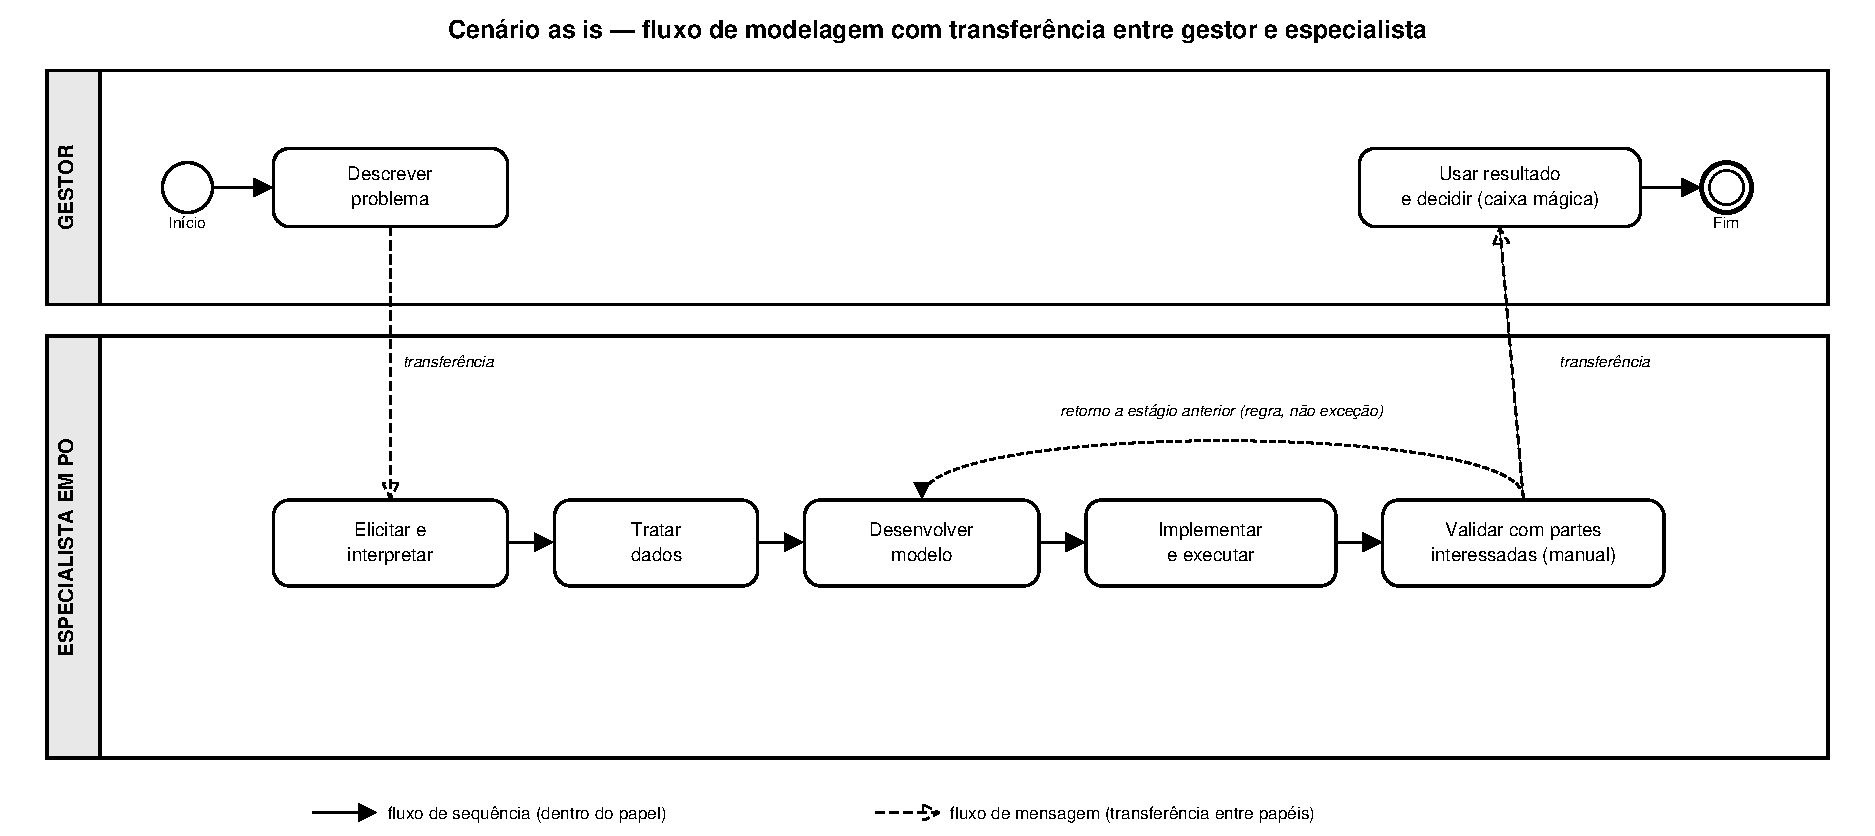
\includegraphics[width=0.95\textwidth]{figuras/fig1_as_is.pdf}
\fontenota{elaborado pelo autor com base em \citeonline{lawless2025} e em notação BPMN conforme \citeonline{dumas2018}}
\end{figure}

O próprio estudo de \citeonline[p.~19]{lawless2025} declara seu limite principal: foram entrevistados apenas especialistas, e as questões de acessibilidade e usabilidade para não especialistas, assim como a perspectiva dos gestores que usam os resultados, ficaram fora do escopo. A lacuna investigada aqui é, portanto, uma agenda deixada em aberto por quem descreveu a prática com mais detalhe.

Resta saber quando a otimização é o instrumento adequado. \citeonline[p.~761]{rosenhead2006} recupera as condições sob as quais a análise tradicional de PO funciona bem: organização estruturada em hierarquia definida; poucos membros analiticamente sofisticados; tarefa bem definida e repetitiva, que gera dados confiáveis; e consenso sobre as prioridades (Greenberger; Crenson; Crissey, 1976 \textit{apud} \citeauthor{rosenhead2006}, \citeyear{rosenhead2006}, p.~761). Onde há muitos atores, interesses em conflito e incertezas difíceis de representar, o instrumento indicado são os métodos de estruturação de problemas, e não um modelo de otimização, automatizado ou não \cite{rosenhead2006}. Este trabalho se restringe às situações que atendem àquelas condições.

\section{Modelos de linguagem e formulação de otimização}
\label{sec:nl2opt}

Os modelos de linguagem de grande porte (\textit{Large Language Models}, LLMs) interpretam texto, geram representações estruturadas e produzem código. Por isso passaram a ser estudados como ponte entre a descrição de um problema e seu modelo matemático, tarefa chamada \textit{Natural Language to Optimization} (NL2Opt). A área ganhou agenda própria em 2022, com a competição NL4Opt, realizada na conferência NeurIPS, que formalizou a tarefa e publicou um conjunto de dados de referência \cite{ramamonjison2023}. Esse conjunto, o LPWP, reúne 1101 problemas anotados de seis domínios, repartidos em 713 de treinamento, 99 de desenvolvimento e 289 de teste \cite{ramamonjison2023}; são enunciados autocontidos, tipicamente com duas a três variáveis e valores numéricos explícitos no próprio texto \cite{mostajabdaveh2024}.

Desde então surgiram abordagens que automatizam partes diferentes do processo. \citeonline{li2023} propuseram um processo em três fases, que identifica as variáveis, classifica objetivo e restrições e gera o modelo de PLIM. \citeonline{mostajabdaveh2024} desenvolveram uma arquitetura multiagente voltada à formulação e à verificação. O OptiMUS formula modelos, gera e depura código e executa \textit{solvers} \cite{ahmaditeshnizi2024, ahmaditeshnizi2026}. \citeonline{astorga2025} trataram a formulação como busca em um espaço de hipóteses de modelagem. OptiTrust e OptiAgent acrescentaram geração de dados verificáveis, agentes especializados e ciclos de correção \cite{lima2025, monteiro2026}.

O OptiAgent \cite{monteiro2026} é o trabalho mais próximo desta proposta. Ele organiza seis agentes sobre um estado compartilhado, com quatro laços de correção e limite de três iterações por laço. Ao menos um laço foi acionado em 27,8\% dos problemas do ComplexOR, 33,1\% do NLP4LP, 55,1\% do LogiOR e 61,4\% do IndustryOR \cite[p.~9]{monteiro2026}. Os autores atribuem os ganhos à divisão da tarefa entre agentes, e não à redação das instruções, e registram duas limitações: cada configuração foi executada uma única vez, sem medir a variabilidade das saídas; e a avaliação isolada de cada agente, assim como a avaliação com usuários não especialistas, ficou como trabalho futuro \cite[p.~11]{monteiro2026}. Medir o efeito isolado de um agente validador é justamente o experimento central deste trabalho.

\section{O que as propostas atuais não resolvem}
\label{sec:lacunas}

Cinco limitações do estado atual definem a lacuna deste trabalho. Nenhuma é inédita isoladamente; o que não se encontrou foi um artefato que trate as cinco em conjunto. No Capítulo 3, cada uma se converte em um requisito de projeto.

\textbf{Usuário.} As propostas se dirigem a quem já domina o formalismo. O OptiMUS-0.3 se apresenta como ferramenta de produtividade para profissionais que conhecem o domínio, reconhecem que o problema cabe em um modelo de PL ou PLIM e conseguem descrevê-lo com precisão; transformar problemas vagos ou incompletos em especificações concretas é, para os próprios autores, questão em aberto \cite{ahmaditeshnizi2026}. O copiloto de decisão proposto por \citeonline{wasserkrug2025}, capaz de dialogar com decisores e produzir modelos verificáveis sem exigir domínio de otimização, é apresentado como visão a alcançar, e não como resultado obtido.

\textbf{Fluxo completo.} Os sistemas cobrem partes do fluxo, em geral da leitura do enunciado à execução do \textit{solver}. O tratamento dos dados, estágio mais custoso da prática, é o menos automatizado, e a explicação ao decisor aparece como saída de texto, e não como etapa com requisitos próprios.

\textbf{Dados.} Nas organizações, os dados já existem antes do modelo: estão em planilhas e extrações de sistemas, com nomes de coluna em vocabulário de negócio, unidades próprias e granularidade que ninguém escolheu pensando em otimizar. Os conjuntos de avaliação recentes já separam a descrição dos valores numéricos --- o NLP4LP reúne 354 problemas, cada um com arquivo de dados, além de sete estudos de caso \cite[p.~7]{ahmaditeshnizi2026} ---, mas o arquivo é construído para a instância. No OptiMUS-0.3, o formato do arquivo é deduzido dos parâmetros extraídos do texto, e o usuário carrega os dados nesse formato ou usa dados gerados aleatoriamente \cite{ahmaditeshnizi2026}. O dado se ajusta ao modelo, e não o contrário. A dificuldade também não é de volume: no caso \textit{Amazon Locker}, o sistema manteve 100\% de formulações corretas em oito níveis de escala, de 3 KB a 935 KB \cite{ahmaditeshnizi2026}. O que falta é associar a grandeza citada no texto à coluna do arquivo que a contém.

\textbf{Idioma.} Os sistemas e conjuntos de avaliação da área foram desenvolvidos em inglês. O principal conjunto multilíngue de raciocínio matemático, o MGSM, traduz 250 problemas para dez idiomas, entre os quais não está o português; e o raciocínio intermediário em inglês frequentemente iguala ou supera o raciocínio no idioma da pergunta \cite{shi2023}. Não se pode supor, portanto, que resultados obtidos em inglês se transfiram para descrições organizacionais em português.

\textbf{Confiabilidade e rastreabilidade.} Código que executa e valor objetivo correto não garantem modelo correto. No exemplo de \citeonline{refai2025}, uma formulação recuperou duas das quatro restrições de referência, omitiu as de integralidade e de capacidade, acrescentou uma restrição inexistente no gabarito e ainda assim atingiu \textit{optimality gap} igual a zero: precisão de 0,67, revocação de 0,50 e erro aparente nulo. O estudo cobre apenas quatro problemas; mostra que o fenômeno existe, mas não com que frequência ocorre. Os próprios gabaritos também falham: na inspeção de \citeonline{xiao2025}, com cada caso validado por ao menos três especialistas, todos os conjuntos de avaliação, exceto o EasyLP, apresentaram erro em mais de 15\% dos problemas, chegando a pelo menos 54\% no IndustryOR. Como as correções automáticas são frequentes (seção~\ref{sec:nl2opt}), o usuário só consegue confiar no resultado se as premissas, os componentes do modelo, as validações e as correções ficarem registrados. Essa rastreabilidade do processo é diferente de expor o texto de raciocínio do modelo de linguagem: a primeira é verificável, porque incide sobre artefatos guardados e comparáveis com a saída final; o segundo não guarda relação garantida com o que foi efetivamente gerado.

\section{Autocorreção e verificação externa em modelos de linguagem}
\label{sec:autocorrecao}

\citeonline{tyen2024} separaram duas capacidades que costumavam ser tratadas juntas: encontrar um erro e corrigi-lo. Os modelos de linguagem testados falharam em localizar erros lógicos, mesmo em casos objetivos; mas, quando recebiam a localização do erro, corrigiam-no bem nas cinco tarefas de raciocínio avaliadas. O gargalo está em localizar, e não em corrigir.

O resultado confirma um diagnóstico anterior. \citeonline{huang2024} mostraram que, em tarefas de raciocínio, os modelos não melhoram ao revisar a própria resposta sem ajuda externa, e podem até piorar. Mostraram também que trabalhos que relatavam ganho usavam a resposta correta para decidir quando parar a revisão, o que não é autocorreção de fato. Em revisão crítica da área, \citeonline{kamoi2024} não encontraram trabalho que demonstre autocorreção bem-sucedida apoiada só na avaliação do próprio modelo.

Uma ressalva: treinamentos específicos e modelos de raciocínio mais recentes já mostram melhor capacidade de autoverificação, de modo que esse limite não é permanente. Para o modelo de uso geral empregado neste trabalho, a consequência de projeto é direta: um verificador deve localizar o erro com sinais externos ao modelo e entregar essa localização para a correção.

  % capitulos/cap3.tex — Capítulo 3 (Metodologia).
% Reescrito em 25/09/2026 no enxugamento pós-feedback (ver
% auditoria/plano_enxugamento.md). Mudanças em relação à versão de
% 29/08/2026 (auditoria/versoes/pre_enxugamento/cap3.tex):
% (1) a antiga seção 3.1 (fluxo atual e os cinco elementos E1-E5) migrou,
%     condensada, para o Capítulo 2 — a Metodologia começa direto no método;
% (2) os oito passos viram seções numeradas em sequência, sem subseções
%     soltas entre eles ("Cenário pretendido" e "Estratégia de avaliação"
%     foram absorvidas por 3.1 e pelo Passo 3);
% (3) siglas reduzidas: E1-E5, I1-I6, C0/C1 e "1e" saem do texto; ficam
%     R1-R5 e, só no quadro próprio, S1-S5;
% (4) limitações reunidas em uma seção única (3.11);
% (5) detalhes cortados ficam guardados para o TG2 (índice em
%     auditoria/plano_enxugamento.md, seção 4).
% Contém: 9 Quadros (eram 14), 1 Tabela, 2 Figuras (fig:fluxo-metodologico,
% fig:to-be; fig4_arquitetura e fig5_sintese retiradas). As equações
% eq:pl/eq:milp passaram para o Capítulo 2.
\chapter{Metodologia}

Este capítulo descreve como a pesquisa será conduzida. A seção~\ref{sec:dsr} caracteriza a pesquisa e apresenta o caminho metodológico, organizado pela \textit{Design Science Research} em oito passos. As seções~\ref{sec:requisitos-projeto} a~\ref{sec:falhas} descrevem os passos na ordem em que são executados; cada um usa o produto do anterior e entrega o que o seguinte precisa. A seção~\ref{sec:piloto} relata o piloto feito nesta etapa, e a seção~\ref{sec:limitacoes} reúne as limitações do desenho.

\section{Caracterização da pesquisa e caminho metodológico}
\label{sec:dsr}

A pesquisa é aplicada quanto à natureza, pois constrói um artefato para um problema organizacional específico; exploratória quanto aos objetivos; quantitativa na etapa de avaliação; e combina pesquisa bibliográfica e experimento quanto aos procedimentos.

O método condutor é a \textit{Design Science Research} (DSR), nas seis etapas de \citeonline{peffers2007}: identificação do problema e motivação, definição dos objetivos da solução, projeto e desenvolvimento, demonstração, avaliação e comunicação. A DSR é o único método do trabalho. A revisão de literatura, a construção do artefato, a demonstração e o experimento são os instrumentos com que cada etapa é realizada. A Figura~\ref{fig:fluxo-metodologico} mostra os oito passos em sequência, e o Quadro~\ref{q:dsr} indica a que etapa da DSR cada passo pertence, o que ele produz e como esse produto é usado adiante.

\begin{figure}[htbp]
\caption{Caminho metodológico: os oito passos e o que cada um produz}
\label{fig:fluxo-metodologico}
\centering
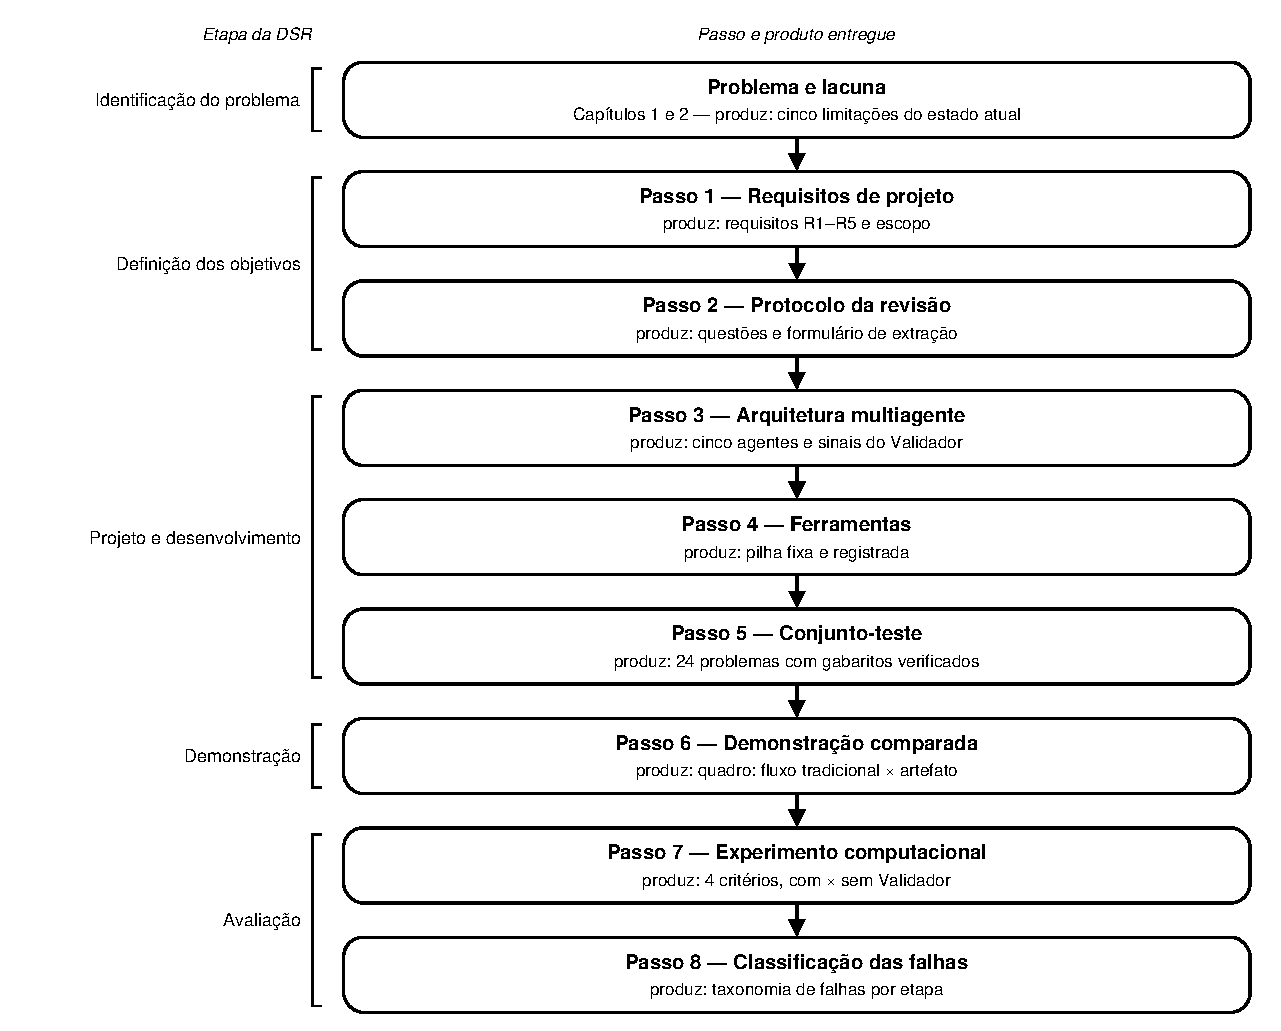
\includegraphics[width=0.9\textwidth]{figuras/fig2_fluxo_metodologico.pdf}
\fontenota{elaborado pelo autor}
\end{figure}

\begin{quadro}[htbp]
\caption{Etapas da DSR e sua realização no trabalho}
\label{q:dsr}
\centering
\small
\begin{tabularx}{\textwidth}{@{}X l X X@{}}
\toprule
Etapa da DSR & Passos & Produto & Uso na etapa seguinte \\
\midrule
Identificação do problema & Caps. 1 e 2 & Cinco limitações do estado atual & Convertidas em requisitos no Passo 1 \\
Definição dos objetivos & 1 e 2 & Requisitos R1--R5; protocolo da revisão & Orientam o desenho da arquitetura \\
Projeto e desenvolvimento & 3, 4 e 5 & Arquitetura, ferramentas e conjunto-teste de 24 problemas & Insumo comum da demonstração e do experimento \\
Demonstração & 6 & Quadro comparativo entre o fluxo tradicional e o artefato & Falhas observadas alimentam o Passo 8 \\
Avaliação & 7 e 8 & Resultados dos quatro critérios; classificação das falhas & Conclusões e trabalhos futuros \\
Comunicação & --- & Documento e apresentação à banca & --- \\
\bottomrule
\end{tabularx}
\fontenota{elaborado pelo autor com base em \citeonline{peffers2007}}
\end{quadro}

No TG1, os Passos 1 a 5 são especificados e um piloto verifica a viabilidade técnica (seção~\ref{sec:piloto}); a construção do artefato e a execução dos Passos 6 a 8 ocorrem no TG2. Os critérios de avaliação são definidos antes da construção porque, na DSR, os objetivos da solução precedem o projeto. Isso também impede que os critérios sejam ajustados depois, conforme o que o artefato conseguir fazer.

Para posicionar a avaliação, adota-se o arcabouço FEDS \cite{venable2016}, na estratégia \textit{Technical Risk \& Efficacy}. Ela é indicada quando o principal risco é técnico e quando é preciso mostrar com rigor que o efeito observado vem do artefato, e não de outro fator \cite[p.~82]{venable2016}. É o caso do experimento, que isola o efeito do agente Validador em ambiente controlado. A demonstração comparada, por sua vez, pertence à etapa de Demonstração da DSR: aplica o artefato a casos concretos e não é um experimento. Sua unidade de análise é o caso resolvido, e não a pessoa que o resolveu.

\section{Passo 1: requisitos de projeto}
\label{sec:requisitos-projeto}

As cinco limitações do estado atual (seção~\ref{sec:lacunas}) convertem-se em cinco requisitos de projeto. O Quadro~\ref{q:requisitos} apresenta cada requisito e onde ele é aferido.

\begin{quadro}[htbp]
\caption{Requisitos de projeto e ponto de aferição}
\label{q:requisitos}
\centering
\small
\begin{tabularx}{\textwidth}{@{}l X l X@{}}
\toprule
Req. & Enunciado & Limitação & Onde é aferido \\
\midrule
R1 & Conduzir a decisão sem exigir do usuário conhecimento de Pesquisa Operacional & Usuário & Demonstração: pré-requisitos e tempo \\
R2 & Percorrer o fluxo completo, da interpretação à explicação, sem intervenção externa & Fluxo completo & Experimento: critério 2; demonstração: ferramentas, etapas e tempo \\
R3 & Obter e associar parâmetros de fontes externas de dados estruturados, pedindo ao usuário o tratamento que faltar & Dados & Experimento: acurácia da associação e critério 2 \\
R4 & Conduzir a interação em língua portuguesa & Idioma & Condição de todo o protocolo \\
R5 & Expor premissas, componentes matemáticos, validações e alterações do processo & Rastreabilidade & Demonstração: relatórios e rastreabilidade; experimento: critério 4 \\
\bottomrule
\end{tabularx}
\fontenota{elaborado pelo autor}
\end{quadro}

O agente Validador não é um sexto requisito: é o mecanismo que realiza R5. Para que as validações e correções fiquem expostas, alguém precisa produzi-las e registrá-las, e esse é o papel do Validador. Como ele é um componente separável, seu efeito pode ser medido, o que transforma uma escolha de arquitetura em hipótese testável (critério 4, seção~\ref{sec:experimento}). É o experimento que os autores do OptiAgent deixaram como trabalho futuro \cite[p.~11]{monteiro2026}.

Com isso, a pergunta de pesquisa fica coberta em duas partes. A primeira --- se a arquitetura produz modelos corretos, executáveis e rastreáveis --- é respondida pelos critérios 1 a 3 do experimento e pela demonstração comparada. A segunda --- qual o efeito do agente validador --- é respondida pelo critério 4.

O escopo é o seguinte: problemas de PL e PLIM em três famílias (alocação de recursos, mistura de insumos e transporte ou distribuição), em organizações que atendem às condições de aplicabilidade da PO descritas na seção~\ref{sec:po-barreira}. Ficam fora problemas não lineares, formulações estocásticas, uso por vários usuários simultâneos e operação em escala de produção.

\section{Passo 2: protocolo da revisão de literatura}
\label{sec:revisao}

A revisão sistemática confirma a lacuna e levanta as arquiteturas concorrentes, informando as decisões do Passo 3; seus resultados ampliarão o Capítulo 2 no TG2. O processo segue as diretrizes de \citeonline{kitchenham2007}, e o relato segue o PRISMA 2020 \cite{page2021}. As questões de revisão são:

\begin{enumerate}[label=QR\arabic*.]
  \item Quais arquiteturas baseadas em modelos de linguagem foram propostas para formular e resolver problemas de otimização, e que etapas do fluxo de modelagem cada uma cobre?
  \item Qual é o público-alvo declarado dessas arquiteturas, e que conhecimento prévio elas pressupõem do usuário?
  \item De onde vêm os parâmetros dos modelos, e em que medida as fontes de dados existem antes do modelo?
  \item Que mecanismos de validação, correção e rastreabilidade essas arquiteturas incorporam, e como seu efeito é avaliado?
\end{enumerate}

No planejamento, definem-se as bases, as expressões de busca e a janela temporal, a partir de 2022. Na condução, aplicam-se critérios de inclusão e exclusão fixados de antemão, com triagem por título e resumo e depois por texto completo. A extração registra, para cada trabalho, uma coluna por limitação da seção~\ref{sec:lacunas}, além da classe de problema, do tipo de avaliação e do número de repetições por instância. O relato traz o fluxograma PRISMA e um quadro comparativo dos trabalhos incluídos. A ferramenta Elicit apoia a triagem e a extração, com conferência manual de todos os itens.

\section{Passo 3: arquitetura multiagente}
\label{sec:arquitetura}

O artefato é um encadeamento de cinco agentes especializados sobre um estado compartilhado. Cada agente recebe uma entrada definida, produz uma saída definida e registra ao menos um artefato que o usuário pode inspecionar. Cada um assume um estágio do fluxo atual de modelagem (seção~\ref{sec:po-barreira}), como mostram a Figura~\ref{fig:to-be} e o Quadro~\ref{q:agentes}.

\begin{figure}[htbp]
\caption{Cenário \textit{to be}: fluxo de modelagem mediado pela plataforma multiagente}
\label{fig:to-be}
\centering
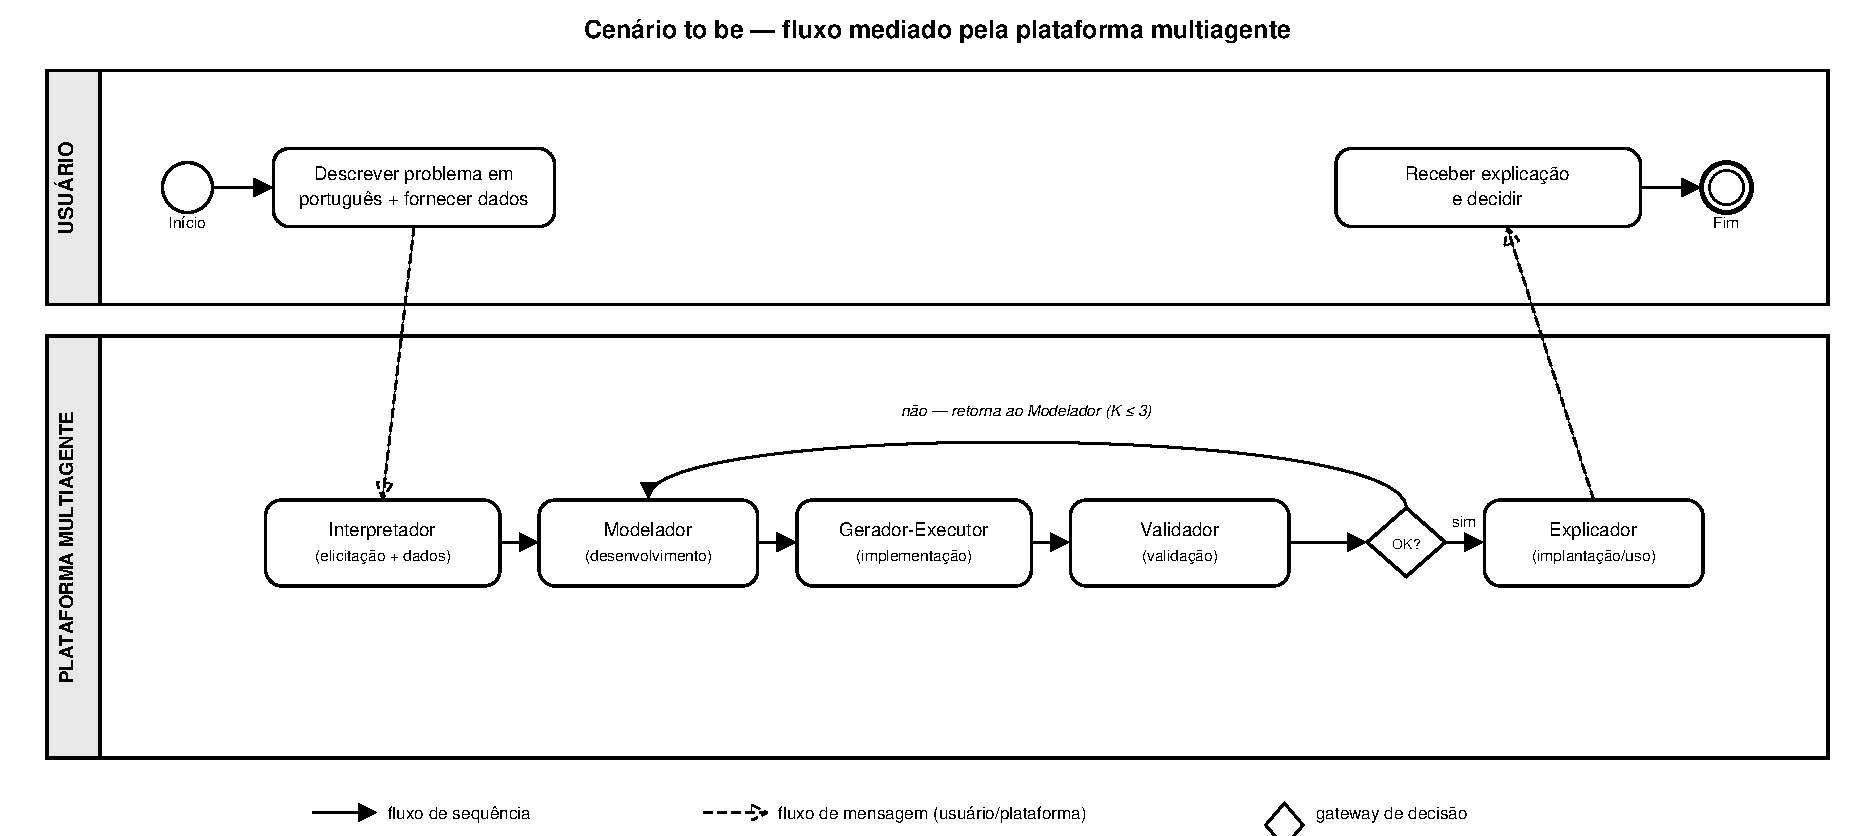
\includegraphics[width=0.95\textwidth]{figuras/fig3_to_be.pdf}
\fontenota{elaborado pelo autor}
\end{figure}

\begin{quadro}[htbp]
\caption{Agentes: estágio assumido, entrada, saída e artefato registrado}
\label{q:agentes}
\centering
\small
\begin{tabularx}{\textwidth}{@{}l X X X@{}}
\toprule
Agente & Estágio do fluxo atual & Entrada $\rightarrow$ saída & Artefato registrado \\
\midrule
Interpretador & Elicitação e tratamento dos dados & Descrição e fontes de dados $\rightarrow$ quadro de especificação & Lista de requisitos; inventário das fontes; solicitações de tratamento e respostas; alertas de ambiguidade \\
Modelador & Desenvolvimento do modelo & Quadro de especificação $\rightarrow$ modelo em JSON & Documento JSON, com o requisito de origem de cada restrição \\
Gerador-Executor & Implementação & JSON $\rightarrow$ código e resultado & Script e registro de execução do \textit{solver} \\
Validador & Validação & JSON, quadro e resultado $\rightarrow$ aprovação ou erro localizado & Registro das validações, com o sinal que originou cada uma \\
Explicador & Implantação e uso & Resultado e artefatos $\rightarrow$ explicação em linguagem de negócio & Explicação final \\
\bottomrule
\end{tabularx}
\fontenota{elaborado pelo autor}
\end{quadro}

\textbf{Interpretador.} Tem duas tarefas. A primeira é converter a descrição em uma lista numerada de requisitos, em vocabulário de negócio, com alerta quando o texto admitir mais de uma leitura. A segunda é obter os parâmetros nas fontes de dados em três operações: ler as fontes e suas colunas sem alterá-las; confrontar cada parâmetro exigido com as colunas disponíveis; e, quando o parâmetro não estiver disponível diretamente, solicitar ao usuário o tratamento necessário, nomeando arquivo, coluna e forma esperada. O artefato não transforma dados: agregação, conversão de unidade, junção de fontes e preenchimento de faltantes ficam com o usuário. Uma transformação silenciosa alteraria todos os números seguintes sem gerar sinal de erro, e o \textit{solver} resolveria corretamente o modelo errado. A solicitação deve tratar do dado, nunca pedir ao usuário que julgue a formulação matemática; nos testes de \citeonline{wasserkrug2025}, o modelo de linguagem pediu a um decisor de negócio que validasse a formulação, pedido que os autores consideraram irrealista.

\textbf{Quadro de especificação.} É a saída do Interpretador e o documento que o usuário lê. Registra, em linguagem de negócio, a decisão a tomar, o critério a otimizar, cada limite declarado, cada parâmetro com sua origem (arquivo, coluna e autorização do usuário, quando houve tratamento) e o que não foi considerado. A estrutura segue o arcabouço de modelagem conceitual de \citeonline{robinson2008a, robinson2008b}, que separa premissas de simplificações; a linha ``não considerado'' torna visíveis as simplificações, onde um modelo costuma deixar de representar a operação sem que ninguém perceba.

\textbf{Representação intermediária.} O Modelador descreve o modelo em um documento JSON, e o Gerador-Executor o traduz em código. Essa separação permite trocar o \textit{solver} sem mudar a formulação e, sobretudo, comparar a formulação com o gabarito componente a componente, independentemente do código (critério 1). Cada restrição guarda o identificador do requisito que a motivou. Adota-se esquema próprio, e não um formato de intercâmbio existente, porque é preciso registrar junto ao modelo a origem de cada parâmetro.

\textbf{Validador e laço de correção.} Como os modelos de linguagem localizam mal os próprios erros, mas os corrigem bem quando recebem sua localização (seção~\ref{sec:autocorrecao}), o Validador é desenhado para localizar. Cada verificação usa um sinal externo, calculável sem que o modelo julgue a própria saída (Quadro~\ref{q:sinais}). O sinal S4, por exemplo, verifica a cobertura dos requisitos por contagem de identificadores, e não por comparação de significado, que seria um juízo do modelo sobre si mesmo. Se o modelo for reprovado, o Validador devolve ao Modelador o elemento com erro, até o limite de três iterações, o mesmo adotado pelo OptiAgent \cite{monteiro2026}. O laço é um retorno à formulação, e não uma nova tentativa após erro de código. Ele para pelo limite fixo e nunca consulta o gabarito, evitando a falha apontada por \citeonline{huang2024}.

\begin{quadro}[htbp]
\caption{Sinais externos do Validador}
\label{q:sinais}
\centering
\small
\begin{tabularx}{\textwidth}{@{}l X X X@{}}
\toprule
\# & Sinal & Como é obtido & O que localiza \\
\midrule
S1 & Estado de retorno do \textit{solver} & Execução, incluindo inviabilidade e ilimitação & Restrições incompatíveis ou insuficientes \\
S2 & Consistência de unidades & Unidades dos parâmetros declaradas no quadro de especificação & Restrição ou termo cujas unidades não fecham \\
S3 & Cobertura de parâmetros & Confronto entre o JSON e o quadro de especificação & Parâmetro usado sem origem declarada \\
S4 & Cobertura de requisitos & Confronto entre os identificadores dos requisitos e os declarados em cada restrição & Requisito sem restrição, ou restrição sem requisito \\
S5 & Limites triviais & Cotas elementares do valor objetivo calculadas a partir dos dados & Solução fora da faixa admitida pelos dados \\
\bottomrule
\end{tabularx}
\fontenota{elaborado pelo autor}
\end{quadro}

\section{Passo 4: ferramentas}
\label{sec:ferramentas}

A arquitetura exige uma ferramenta para cada componente (Quadro~\ref{q:ferramentas}). A pilha fica fixa durante todo o trabalho, o que é condição para reproduzir os Passos 5 a 7.

\begin{quadro}[htbp]
\caption{Ferramentas selecionadas}
\label{q:ferramentas}
\centering
\small
\begin{tabularx}{\textwidth}{@{}l l X@{}}
\toprule
Camada & Escolha & Justificativa \\
\midrule
Modelagem & PuLP e Pyomo & Modelagem em Python independente do \textit{solver} \cite{mitchell2011, hart2011} \\
\textit{Solver} & CBC 2.10.3 \cite{forrest2019} & Código aberto, distribuído com o PuLP, sem licença comercial; usado no piloto \\
\textit{Solver} alternativo & SCIP \cite{achterberg2009} & Contingência, caso o CBC seja insuficiente em PLIM \\
Modelo de linguagem & Acesso por API & Versão, temperatura e parâmetros de inferência registrados \\
Orquestração & Grafo de estados & Explicita nós e o retorno do laço, o que permite remover o Validador \\
Interface & A definir no TG2 & Deve exibir o modelo e os artefatos intermediários (R5) \\
\bottomrule
\end{tabularx}
\fontenota{elaborado pelo autor}
\end{quadro}

O \textit{solver} é definido em um único ponto do código, fica idêntico nas duas configurações do experimento e não é escolhido pelo modelo de linguagem; nome e versão são registrados em cada execução. Na interface, o Streamlit foi descartado por não exibir os objetos do modelo, o que o torna incompatível com R5.

\section{Passo 5: construção do conjunto-teste}
\label{sec:conjunto-teste}

O conjunto-teste é o insumo comum da demonstração (Passo 6) e do experimento (Passo 7). Reúne 24 problemas: três famílias (alocação, mistura e transporte ou distribuição), duas classes (PL e PLIM) e quatro problemas por combinação (3 $\times$ 2 $\times$ 4 = 24). Cada instância tem seis componentes:

\begin{enumerate}[label=\alph*)]
  \item descrição do problema em português, no registro de um gestor, sem termos de Pesquisa Operacional;
  \item uma ou mais fontes de dados externas à descrição, com nomes de coluna em vocabulário operacional; ao menos um terço das instâncias deve exigir solicitação de tratamento, por granularidade, unidade ou identificador divergente;
  \item formulação matemática de referência;
  \item código de referência executável;
  \item solução e valor objetivo verificados por \textit{solver};
  \item gabarito de associação entre parâmetros e colunas e, quando for o caso, as solicitações de tratamento esperadas.
\end{enumerate}

A família de um problema é decidida pela estrutura da formulação de referência, e não pelas palavras do enunciado. É alocação quando se atribuem recursos escassos a atividades concorrentes; mistura quando se definem proporções de insumos sujeitas a especificações; e transporte ou distribuição quando há fluxo entre origens e destinos sujeito a oferta e demanda.

A construção segue esta ordem: escolha da origem (adaptação de problemas de \citeonline{arenales2007} ou construção própria); redação da descrição em linguagem de negócio; separação dos parâmetros em arquivo externo; formulação de referência feita sem usar o artefato; verificação da solução por \textit{solver}; e revisão cruzada dos gabaritos por terceiro. Os conjuntos públicos não são usados diretamente porque contêm erros de gabarito (seção~\ref{sec:lacunas}); em um experimento que busca isolar o efeito do Validador, um gabarito errado confundiria o efeito com ruído.

Duas ameaças são tratadas nesta etapa. A primeira é a contaminação: problemas de livro-texto podem estar nos dados de treinamento dos modelos de linguagem, e \citeonline[p.~9]{monteiro2026} observam que conjuntos mais antigos produzem escores mais altos. Por isso, parte das instâncias é de construção própria, as adaptadas têm contexto, unidades e valores alterados, e os resultados são reportados separadamente para os dois grupos. A segunda é o conflito de papéis, já que o autor do artefato também escreve os gabaritos; a formulação de referência é feita antes de qualquer execução do artefato e revisada por terceiro.

O conjunto também fornece os casos da demonstração comparada: problemas já resolvidos pelo fluxo tradicional em exercícios e estudos de caso de disciplina, acrescidos, se possível, de um caso real, que entra como instância zero e serve de referência de estilo para as demais descrições. O caso real deve ser de PL ou PLIM em uma das três famílias, ter dados em arquivo real com vocabulário de negócio, ser resolúvel pelo fluxo tradicional no prazo e ter gabarito verificável; as fontes possíveis são a empresa júnior da universidade, um contato de estágio ou a própria operação da universidade. De cada caso registram-se apenas o enunciado com os dados, a resolução (modelo, ferramenta e etapas) e o resultado. Nada é registrado sobre quem resolveu, o que dispensa submissão a comitê de ética em pesquisa.

\section{Passo 6: demonstração comparada}
\label{sec:demonstracao}

Este passo usa os casos do Passo 5 para comparar o que o fluxo tradicional exige e entrega com o que o artefato exige e entrega, atendendo ao quinto objetivo específico. Fluxo tradicional é o praticado no ensino e na prática de PO: ler o enunciado, formular o modelo à mão, implementá-lo em planilha com o Solver do Excel ou em \textit{solver} dedicado e ler os relatórios de saída. A comparação usa os seis indicadores do Quadro~\ref{q:indicadores}.

\begin{quadro}[htbp]
\caption{Indicadores da demonstração comparada}
\label{q:indicadores}
\centering
\small
\begin{tabularx}{\textwidth}{@{}l X X l@{}}
\toprule
Indicador & Fluxo tradicional & Artefato & Req. \\
\midrule
Pré-requisitos & Formular o modelo, reconhecer a classe do problema e operar a ferramenta & Descrever a decisão em português & R1 \\
Ferramentas & Quantas e quais (planilha, Solver do Excel, \textit{solver} dedicado etc.) & Quantas e quais & R2 \\
Etapas & Passos manuais e trocas de ferramenta & Passos manuais e trocas de ferramenta & R2 \\
Tempo & Ordem de grandeza registrada no caso & Ordem de grandeza registrada & R1, R2 \\
Relatórios & Solução, valor objetivo, sensibilidade, preços-sombra, folgas, limites & Presença ou ausência de cada item & R5 \\
Rastreabilidade & O que fica inspecionável: modelo, parâmetros e origem, validações & O que fica inspecionável & R5 \\
\bottomrule
\end{tabularx}
\fontenota{elaborado pelo autor}
\end{quadro}

Os indicadores são descritivos (presença, ausência, contagem e ordem de grandeza) e não sustentam inferência estatística. O tempo é o indicador mais frágil: no artefato mede processamento e, no fluxo tradicional, trabalho humano, por isso é reportado só como ordem de grandeza. O indicador de relatórios deve desfavorecer o artefato: o Solver do Excel gera relatórios de respostas, de sensibilidade e de limites \cite{frontlinesystems2024}, e o protótipo previsto não gera preços-sombra nem custos reduzidos. Esse resultado será relatado como limitação. Quais casos entram na demonstração, em que número e de que fonte será definido no TG2.

\section{Passo 7: experimento computacional}
\label{sec:experimento}

O experimento mede os quatro critérios do Quadro~\ref{q:criterios} em delineamento pareado: as 24 instâncias são executadas em duas configurações, \textbf{com Validador} (fluxo completo) e \textbf{sem Validador}. Na configuração sem Validador, o agente é removido e a saída do Gerador-Executor vai direto ao Explicador; executá-lo e ignorar seu parecer mediria outra coisa, pois manteria o custo e alteraria o estado compartilhado. Ficam idênticos nas duas configurações o modelo de linguagem e sua versão, a temperatura e demais parâmetros de inferência, as instruções dos outros agentes, a representação intermediária, o \textit{solver} e as instâncias. Para evitar que uma atualização do modelo pelo fornecedor contamine a comparação, as configurações são executadas de forma intercalada por instância, com data e hora registradas.

Cada instância é executada três vezes em cada configuração e contada como correta quando acerta em pelo menos duas. A repetição responde à execução única do OptiAgent \cite[p.~11]{monteiro2026} e ao estudo de estabilidade do OptiMUS-0.3, em que dez de quinze instâncias difíceis alternaram entre acerto e erro conforme a semente \cite{ahmaditeshnizi2026}.

\begin{quadro}[htbp]
\caption{Critérios de avaliação do experimento computacional}
\label{q:criterios}
\centering
\small
\begin{tabularx}{\textwidth}{@{}l X@{}}
\toprule
Critério & Definição operacional \\
\midrule
1. Acurácia da formulação & Precisão e revocação por componente (variáveis, função objetivo, restrições, domínios e coeficientes), mais a acurácia da associação entre parâmetros e colunas, reportada à parte \\
2. Resolução de ponta a ponta & Proporção de instâncias em que o fluxo interpreta, formula, gera código executável e resolve sem intervenção externa \\
3. Correção da solução & Solução viável, valor objetivo dentro da tolerância e, quando houver gabarito, valores das variáveis corretos \\
4. Efeito do Validador & Diferença entre as configurações nos critérios 1 a 3, número de iterações do laço, proporção de instâncias em que ele foi acionado e sinais que o acionaram \\
\bottomrule
\end{tabularx}
\fontenota{elaborado pelo autor}
\end{quadro}

\textbf{Critério 1.} A formulação é avaliada por componente porque uma métrica agregada esconde erros estruturais (seção~\ref{sec:lacunas}). Para cada componente $k$:

\begin{equation*}
  \text{precisão}(k) = \frac{\mathrm{VP}(k)}{\mathrm{VP}(k) + \mathrm{FP}(k)}, \qquad
  \text{revocação}(k) = \frac{\mathrm{VP}(k)}{\mathrm{VP}(k) + \mathrm{FN}(k)}
\end{equation*}

em que $\mathrm{VP}(k)$ são os elementos do gabarito gerados corretamente, $\mathrm{FP}(k)$ os elementos gerados sem correspondente no gabarito e $\mathrm{FN}(k)$ os elementos do gabarito não gerados. Como duas formulações diferentes podem estar ambas corretas, os elementos são comparados sem depender de ordem ou nome, as restrições são normalizadas (sentido da desigualdade, lado dos termos e escala) e uma restrição agregada é aceita quando equivale a um conjunto de restrições desagregadas. Mesmo assim, o critério mede semelhança com a referência e é um limite inferior da correção, complementado pelo critério 3 \cite{ahmaditeshnizi2026}. Para a comparação entre configurações, a formulação é considerada \textbf{correta} apenas quando precisão e revocação valem 1 em todos os componentes.

A acurácia da associação mede se cada parâmetro foi ligado à coluna certa. Sendo $G$ os pares (parâmetro, coluna) do gabarito e $P$ os pares produzidos pelo artefato, a precisão é $|P \cap G|/|P|$ e a revocação é $|P \cap G|/|G|$; associação a coluna parecida, porém errada, conta como erro. Ela é reportada em separado porque esse erro é silencioso: o modelo executa e devolve um número plausível. Em problema análogo, a ligação entre texto e esquema de banco de dados mostrou-se o ponto crítico da conversão de linguagem natural em consultas \cite{lei2020}.

\textbf{Critério 3.} A solução é correta quando o código executa, o valor objetivo atende a
\begin{equation*}
  |f_{\mathrm{art}} - f_{\mathrm{ref}}| \leq \varepsilon \cdot |f_{\mathrm{ref}}|, \quad \text{com } \varepsilon = 0{,}01,
\end{equation*}
e, quando o gabarito inclui a solução, os valores das variáveis coincidem \cite{ahmaditeshnizi2026}. Aqui, $f_{\mathrm{art}}$ é o valor produzido pelo artefato e $f_{\mathrm{ref}}$ o valor de referência. A tolerância de 1\% segue o OptiMUS-0.3 e é deliberadamente estreita: em PL, uma formulação errada tende a levar a outro vértice, cujo valor pode diferir pouco do ótimo. O valor foi fixado antes de qualquer coleta e não será revisto.

\textbf{Análise estatística.} A análise principal é descritiva: proporções e contagens de cada critério em cada configuração. Como análise secundária, aplica-se o teste de McNemar exato, separadamente aos critérios 1, 2 e 3, sobre as instâncias em que as configurações divergem (células $b$ e $c$ da Tabela~\ref{t:mcnemar}). A versão exata é usada porque 24 instâncias não justificam a aproximação assintótica. Os valores de $b$ e $c$ são sempre reportados com o valor-p. Um efeito nulo do Validador é resultado válido e será relatado como tal.

\begin{table}[htbp]
\caption{Organização dos pares para o teste de McNemar}
\label{t:mcnemar}
\centering
\begin{tabular}{@{}l l l@{}}
\toprule
 & Sem Validador correto & Sem Validador incorreto \\
\midrule
Com Validador correto   & $a$ & $b$ \\
Com Validador incorreto & $c$ & $d$ \\
\bottomrule
\end{tabular}
\fontenota{elaborado pelo autor com base em \citeonline{mcnemar1947}}
\end{table}

O Quadro~\ref{q:reprodutibilidade} reúne as condições necessárias para que terceiros reproduzam o experimento e a demonstração.

\begin{quadro}[htbp]
\caption{Síntese de reprodutibilidade}
\label{q:reprodutibilidade}
\centering
\small
\begin{tabularx}{\textwidth}{@{}X X l@{}}
\toprule
Condição & Resposta & Seção \\
\midrule
Quantos problemas & 24 (3 famílias $\times$ 2 classes $\times$ 4) & \ref{sec:conjunto-teste} \\
Como são obtidos & Adaptação de \citeonline{arenales2007} e construção própria & \ref{sec:conjunto-teste} \\
Como se classifica a família & Pela estrutura da formulação de referência & \ref{sec:conjunto-teste} \\
Execuções por problema & 3 por configuração, com decisão por maioria & \ref{sec:experimento} \\
Configurações comparadas & Com Validador e sem Validador (agente removido) & \ref{sec:experimento} \\
O que fica constante & Modelo de linguagem e versão, parâmetros de inferência, instruções, JSON, \textit{solver} e instâncias & \ref{sec:experimento} \\
Como se calcula a acurácia & Precisão e revocação por componente & \ref{sec:experimento} \\
Quando a formulação é correta & Precisão = revocação = 1 em todos os componentes & \ref{sec:experimento} \\
Como se registra uma falha & Pela etapa em que a divergência aparece primeiro & \ref{sec:falhas} \\
Como se compara com e sem Validador & Pares nas mesmas instâncias; McNemar exato por critério & \ref{sec:experimento} \\
\bottomrule
\end{tabularx}
\fontenota{elaborado pelo autor}
\end{quadro}

\section{Passo 8: classificação dos modos de falha}
\label{sec:falhas}

O último passo classifica as falhas observadas nos Passos 6 e 7 pela etapa em que surgiram (Quadro~\ref{q:taxonomia}). Essa análise mostra onde o artefato falha e compensa, em parte, o baixo poder estatístico do experimento.

\begin{quadro}[htbp]
\caption{Taxonomia dos modos de falha}
\label{q:taxonomia}
\centering
\small
\begin{tabularx}{\textwidth}{@{}l X X@{}}
\toprule
Categoria & Falha & Como se identifica \\
\midrule
Interpretação & Requisito omitido, acrescentado ou com sentido alterado & Lista de requisitos diverge do enunciado \\
Parametrização & Parâmetro ligado à fonte ou coluna errada, ou não ligado & Quadro de especificação diverge do gabarito de associação \\
Solicitação de tratamento & Solicitação necessária não emitida, incompleta ou que pede juízo sobre a formulação & Solicitações emitidas divergem das esperadas \\
Formulação & Variável, restrição, objetivo, domínio ou coeficiente incorreto & JSON diverge do gabarito, com requisitos e dados corretos \\
Geração de código & Código não corresponde ao JSON ou não compila & Código diverge do JSON correto \\
Execução & Erro em tempo de execução ou não convergência & Código correto, falha no ambiente \\
Validação: erro aprovado & Validador aprovou modelo errado & Instância incorreta com Validador, sem acionar o laço \\
Validação: correção indevida & Validador alterou modelo que estava correto & Instância correta antes do laço e incorreta depois \\
Interação & Descrição do usuário que o Interpretador não resolve & Só nos casos da demonstração \\
\bottomrule
\end{tabularx}
\fontenota{elaborado pelo autor}
\end{quadro}

Cada falha é atribuída à primeira etapa em que a divergência aparece, mantidas corretas as anteriores; o encadeamento é registrado à parte. Assim, uma falha de interpretação não é contada também como falha de formulação.

\section{Piloto de aplicação}
\label{sec:piloto}

Nesta etapa, aplicou-se o fluxo completo, uma vez e sem laço de correção, a um problema de PL de alocação de recursos produtivos, com descrição em português e parâmetros em arquivo separado. A formulação de referência e a solução ótima foram obtidas de forma independente por \textit{solver}. O piloto verifica a viabilidade técnica; não é amostra e não gera métrica.

A ocorrência mais relevante foi esta: o modelo de linguagem produziu a formulação correta, mas afirmou uma solução ótima que não correspondia ao próprio modelo, com valor objetivo bem abaixo do ótimo verificado. Solicitado a revisar a saída, justificou o resultado em vez de corrigi-lo. O episódio sustenta duas decisões deste capítulo: avaliar a formulação separadamente da solução (critério 1) e apoiar o Validador em sinais externos, e não na autoavaliação do modelo (seção~\ref{sec:arquitetura}). Em consequência, três ajustes foram incorporados: a solução passou a vir sempre do \textit{solver}, nunca do modelo de linguagem; o \textit{solver} passou a ser fixo; e a temperatura de inferência foi reduzida.

O piloto usou um arquivo de dados fabricado, com nomes de coluna que correspondem diretamente às grandezas do texto. Por isso, ele não testa R3; esse teste depende das instâncias com dados em vocabulário operacional previstas no Passo 5.

\section{Limitações e escopo}
\label{sec:limitacoes}

As limitações do desenho, reunidas aqui, são:

\begin{enumerate}[label=\alph*)]
  \item não há estudo com usuários: usabilidade, confiança, adoção e a capacidade de um usuário detectar erros a partir dos artefatos inspecionáveis não são avaliadas. O trabalho mostra que esses artefatos existem e o que contêm, e deixa a avaliação com usuários para estudos posteriores;
  \item o português é condição do experimento, e não objeto dele: sem comparação com outro idioma, o efeito do idioma sobre o desempenho não é isolado;
  \item com 24 instâncias, o teste estatístico pode não ter poder para detectar diferenças; a análise descritiva é a principal;
  \item três execuções por instância, e não cinco como no OptiMUS-0.3, reduzem a sensibilidade a instâncias instáveis; a escolha decorre de custo e prazo;
  \item o autor do artefato também constrói os gabaritos, risco atenuado pelas medidas do Passo 5;
  \item o critério 1 é um limite inferior da correção, pois pode penalizar formulações alternativas válidas;
  \item o protótipo não gera análise de sensibilidade, embora o \textit{solver} adotado forneça essa informação;
  \item o artefato transfere ao usuário a preparação dos dados; esse trabalho já existia no fluxo tradicional, mas passa a ser explícito e antecipado;
  \item o Interpretador trata a descrição recebida como representação suficiente do problema, a mesma premissa da PO tradicional criticada pelos métodos de estruturação de problemas \cite{rosenhead2006} e adotada pelo OptiMUS-0.3 \cite{ahmaditeshnizi2026}.
\end{enumerate}


\postextual
  % .bst local, não o do sistema (R-3, achado C2/Fase 8, ver
  % auditoria/log.md §19 e o cabeçalho de latex/bst/abntex2-alf-tg1.bst):
  % abntex2cite já dispara \bibliographystyle{abntex2-alf} sozinho via
  % \AtEndDocument se nada for chamado antes — chamar aqui, no corpo, depois
  % de \begin{document}, garante que esta escolha vença a automática.
  \bibliographystyle{latex/bst/abntex2-alf-tg1}
  \bibliography{referencias}

\end{document}
